\section{Zusammenfassung der Ergebnisse}\label{sec:ueberblick}

Für jeden der 13 untersuchten Modelle wurden fünf unabhängige Läufe mit unterschiedlichen Seeds durchgeführt. Abbildung \ref{fig:results-evaluation-metrics-comparison} visualisiert die mittleren Werte für Precision, Recall, F1-Score und Accuracy jeweils inklusive Standardabweichung über alle Wiederholungen hinweg. Für einen besseren Vergleich sind proprietäre Modelle rot, kleinere Modelle orange und größere Modelle blau eingefärbt. Die Einteilung entspricht der in Kapitel~\ref{ch:modellauswahl} beschriebenen Kategorisierung.

\begin{figure}[htbp]
    \centering
    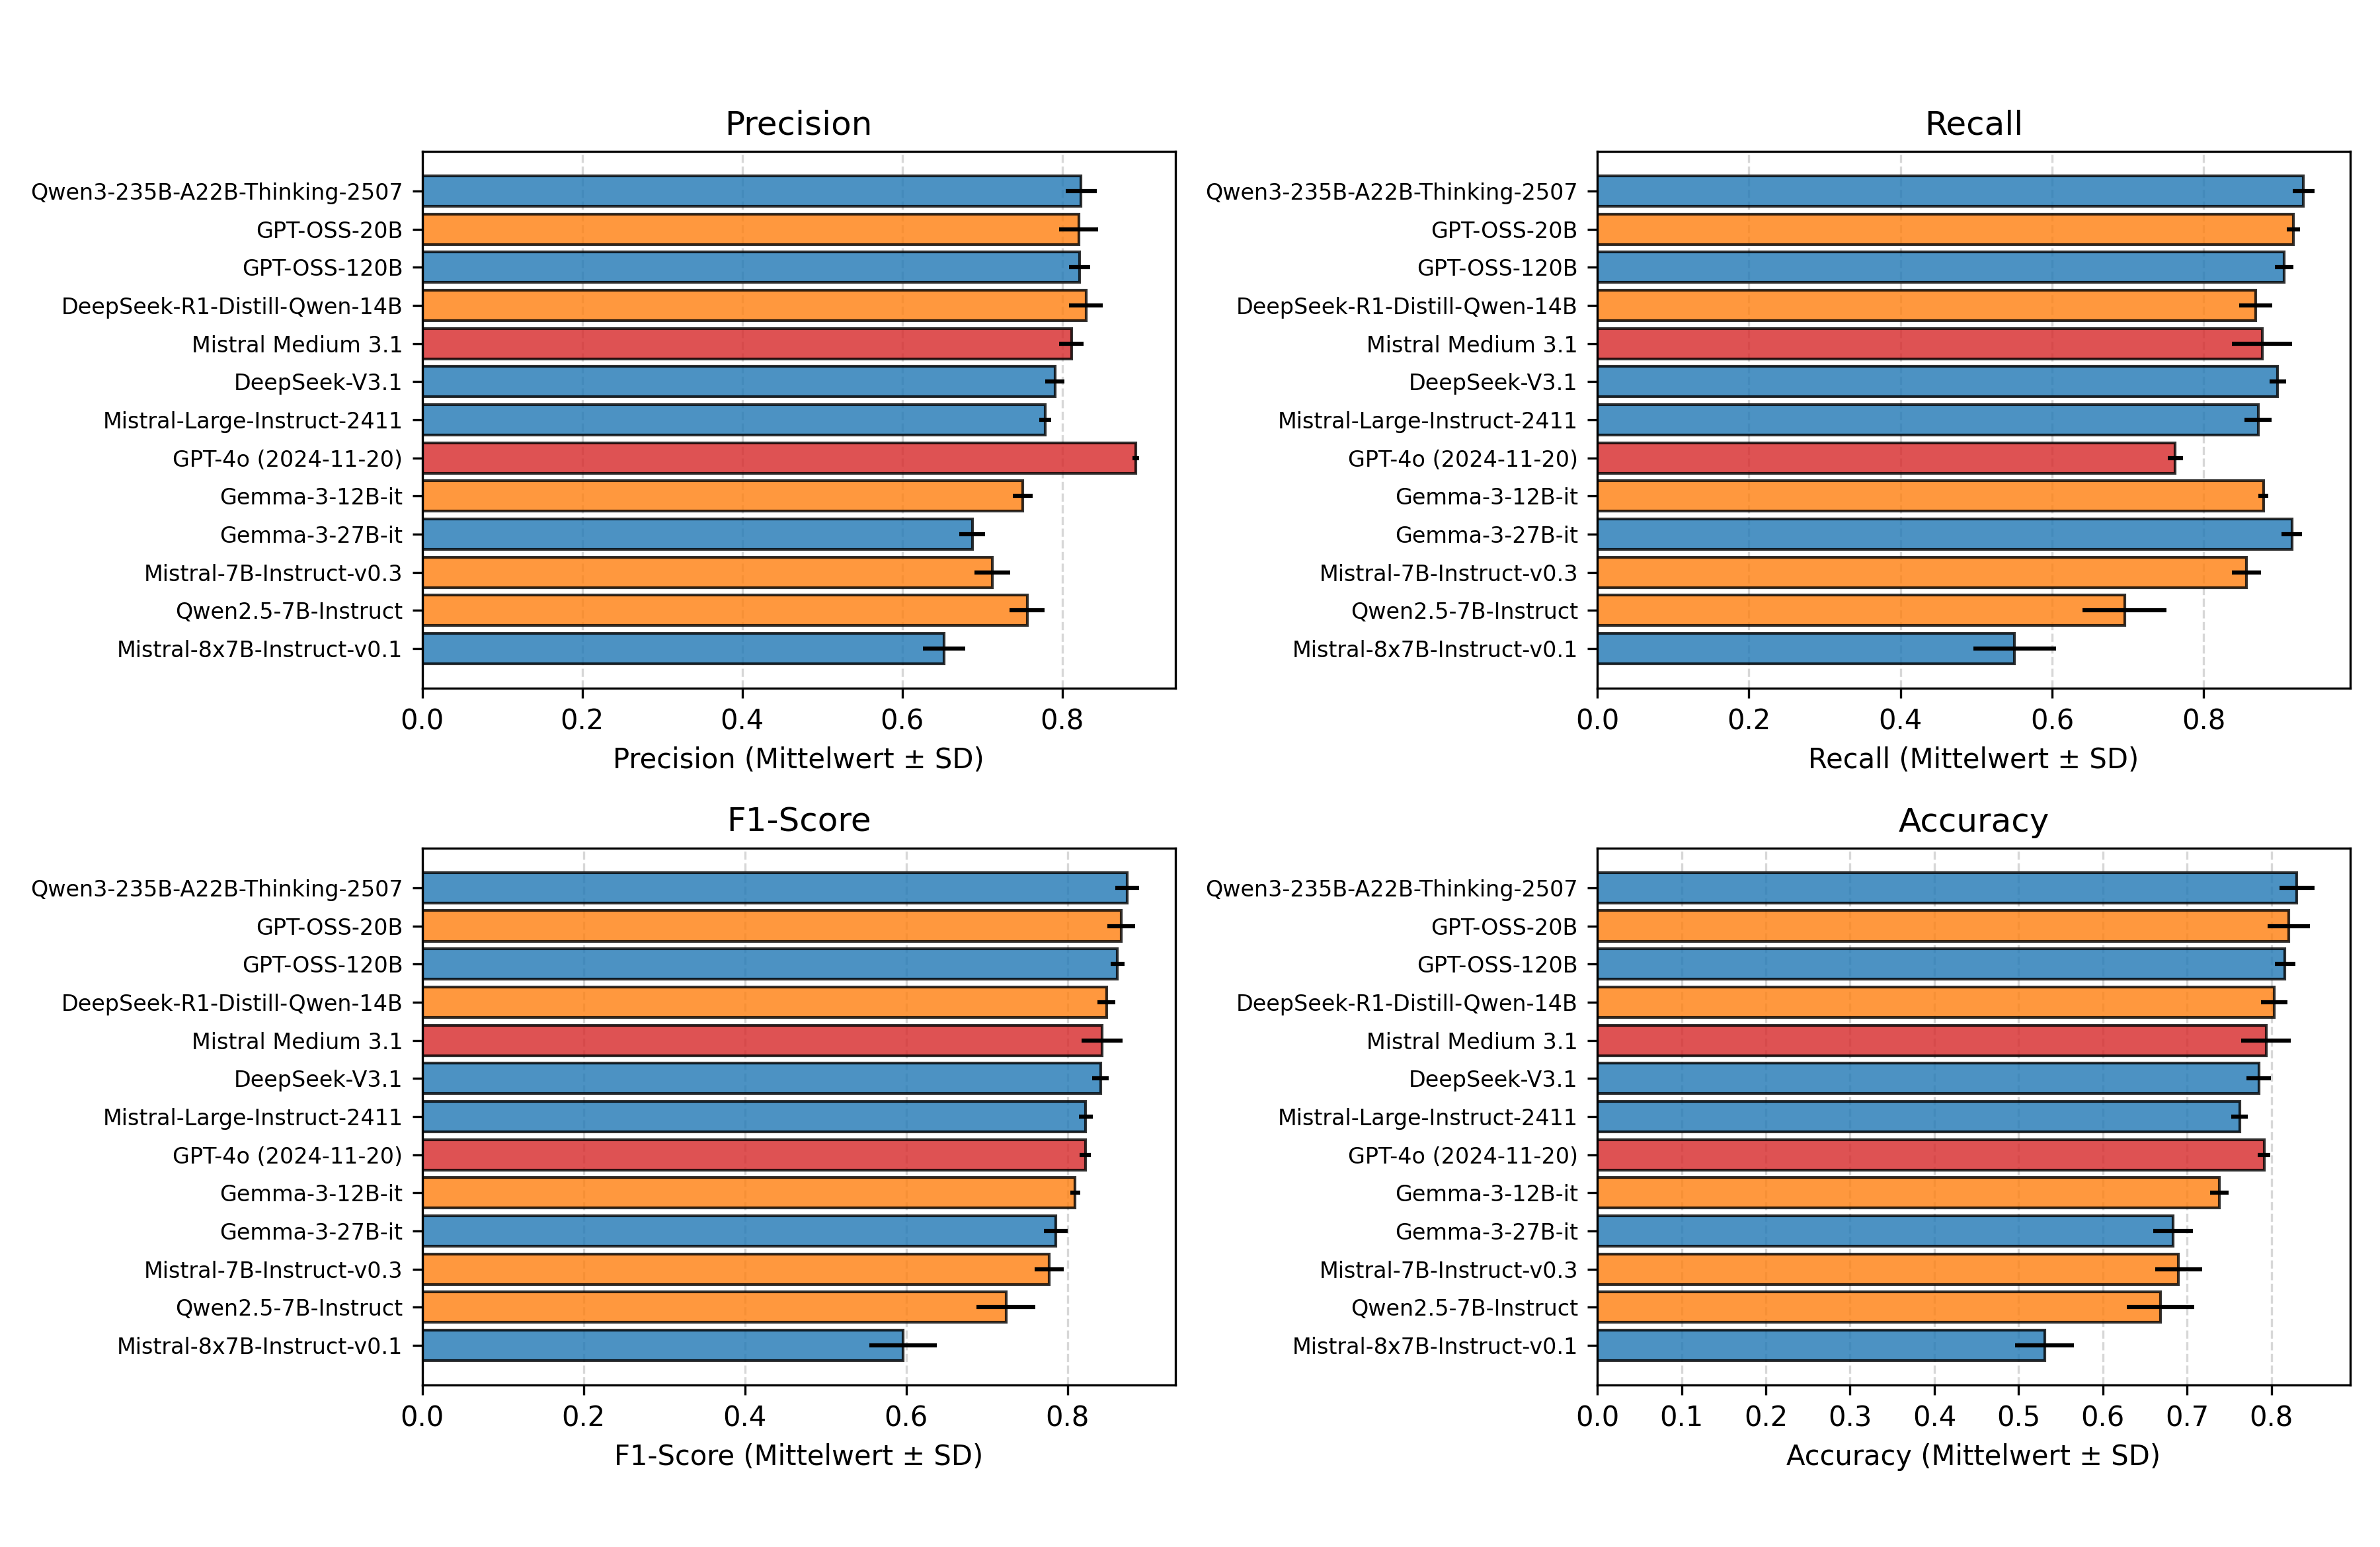
\includegraphics[width=\textwidth,trim=20 40 20 10]{images/results/evaluation_metrics_comparison}
    \caption{Durchschnittliche Metrik-Werte der untersuchten Modelle über alle Wiederholungen hinweg inklusive Standardabweichung.}
    \label{fig:results-evaluation-metrics-comparison}
\end{figure}

Insgesamt erfüllen neun der dreizehn Modelle den Zielwert von $F1-Score \geq 0{,}80$ aus Abschnitt~\ref{sec:qualitatsziele}. Besonders gut schneiden \texttt{Qwen3-235B-A22B-Thinking-2507}, \texttt{GPT-OSS-120B} und \texttt{GPT-OSS-20B} ab, die F1-Scores zwischen $0{,}862$ und $0{,}874$ erreichen. Erfreulich ist, dass auch mehrere kleinere Modelle diesen Zielwert überschreiten. Am unteren Ende des Spektrums liegt das europäische \texttt{Mixtral-8x7B-\linebreak~Instruct-v0.1}, das sowohl in Precision als auch in Recall schwach abschneidet und als einziges Modell einen F1-Score deutlich unter $0{,}60$ erzielt.

Die Abbildung zeigt zudem, dass sich die Modelle hinsichtlich Precision und Recall unterschiedlich verhalten. \texttt{GPT-4o} erreicht beispielsweise mit $0{,}892$ die höchste Precision, liegt jedoch beim Recall mit $0{,}762$ unter dem Mindestziel von $0{,}80$. Umgekehrt erzielt \texttt{Gemma-3-27B-it} einen sehr hohen Recall von $0{,}916$, wird aber durch eine niedrige Precision von $0{,}687$ ausgebremst. Modelle wie \texttt{Qwen3-235B-A22B-\linebreak~Thinking-2507}, \texttt{GPT-OSS-20B} und \texttt{DeepSeek-R1-Distill-Qwen-14B} bieten eine ausgewogene Balance und zählen deshalb zu den Spitzenreitern.

Tabelle \ref{tab:metrics-overview} fasst alle Metriken mit ihren Mittelwerten und Standardabweichungen tabellarisch zusammen. Für die weitere Analyse werden diese Werte nur noch punktuell zitiert, um Wiederholungen zu vermeiden.

\begin{table}[htbp]
    \centering
    \caption{Aggregierte Mittelwerte und Standardabweichungen der Evaluationsmetriken über alle fünf Wiederholungen hinweg.}
    \label{tab:metrics-overview}
    \begin{adjustbox}{width=\textwidth}
        \begin{tabular}{l r r r r}
            \toprule
            Modell                          & Precision         & Recall            & F1-Score          & Accuracy \\
            \midrule
            DeepSeek-V3.1                   & 0.791 $\pm$ 0.012 & 0.897 $\pm$ 0.011 & 0.841 $\pm$ 0.011 & 0.785 $\pm$ 0.015 \\
            DeepSeek-R1-Distill-Qwen-14B    & 0.829 $\pm$ 0.021 & 0.868 $\pm$ 0.022 & 0.848 $\pm$ 0.011 & 0.803 $\pm$ 0.016 \\
            Gemma-3-12B-it                  & 0.751 $\pm$ 0.013 & 0.879 $\pm$ 0.006 & 0.810 $\pm$ 0.006 & 0.738 $\pm$ 0.011 \\
            Gemma-3-27B-it                  & 0.687 $\pm$ 0.016 & 0.916 $\pm$ 0.014 & 0.785 $\pm$ 0.015 & 0.683 $\pm$ 0.023 \\
            Mistral-7B-Instruct-v0.3        & 0.712 $\pm$ 0.022 & 0.856 $\pm$ 0.019 & 0.777 $\pm$ 0.018 & 0.690 $\pm$ 0.028 \\
            Mixtral-8x7B-Instruct-v0.1      & 0.652 $\pm$ 0.027 & 0.550 $\pm$ 0.054 & 0.596 $\pm$ 0.042 & 0.531 $\pm$ 0.035 \\
            Mistral-Large-Instruct-2411     & 0.779 $\pm$ 0.008 & 0.872 $\pm$ 0.018 & 0.823 $\pm$ 0.008 & 0.762 $\pm$ 0.010 \\
            Mistral Medium 3.1              & 0.811 $\pm$ 0.015 & 0.877 $\pm$ 0.040 & 0.843 $\pm$ 0.025 & 0.794 $\pm$ 0.029 \\
            GPT-OSS-20B                     & 0.820 $\pm$ 0.024 & 0.918 $\pm$ 0.009 & 0.866 $\pm$ 0.017 & 0.821 $\pm$ 0.025 \\
            GPT-OSS-120B                    & 0.822 $\pm$ 0.013 & 0.906 $\pm$ 0.012 & 0.862 $\pm$ 0.009 & 0.816 $\pm$ 0.012 \\
            GPT-4o                          & 0.892 $\pm$ 0.004 & 0.762 $\pm$ 0.010 & 0.822 $\pm$ 0.007 & 0.791 $\pm$ 0.007 \\
            Qwen2.5-7B-Instruct             & 0.756 $\pm$ 0.022 & 0.696 $\pm$ 0.055 & 0.724 $\pm$ 0.037 & 0.668 $\pm$ 0.040 \\
            Qwen3-235B-A22B-Thinking-2507   & 0.824 $\pm$ 0.019 & 0.932 $\pm$ 0.014 & 0.874 $\pm$ 0.015 & 0.830 $\pm$ 0.021 \\
            \bottomrule
        \end{tabular}
    \end{adjustbox}
\end{table}